\documentclass[../main.tex]{subfiles}
\graphicspath{{\subfix{../images/}}}
\begin{document}

%%%%%%%%%%%%%%%%%%%%%%%%%%%%%%%%%%%%%%%%%%%%%%%%%%%%%%%%%%%%%%%%%%%%%%%%%%%%%%%%
\section{Знакомство со средой разработки Arduino}
Среда разработки Arduino (Arduino IDE) состоит из встроенного текстового
редактора программного кода, области сообщений, окна вывода текста (консоли),
панели инструментов с кнопками часто используемых команд и нескольких меню. Для
загрузки программ и связи с компьютером среда разработки подключается к
аппаратной части Arduino.

Скачать среду разработки можно с официального сайта Arduino:
\url{https://www.arduino.cc/en/Main/Software}.

Перед скачиванием будет предложено пожертвовать денег проекту Arduino для
дальнейшего развития, но этот шаг необязателен и может быть выполнен на ваше
усмотрение.

После скачивания необходимо установить программу на вашу операционную систему.
Самый простой способ установки на GNU/Linux -- это скачивание архива и его
последующая распаковка в удобный для вас каталог.  В архиве содержится всё
необходимое для запуска Arduino IDE.

Если ваша операционная система настроена на использование русского языка в
интерфейсе, то скорее всего интерфейс Arduino IDE будет русифицирован, как
показано на рис. \ref{fig:arduino-ide-main-window-ru}.

\begin{figure}[ht]
  \centering
  \caption{Главное окно Arduino IDE.}
  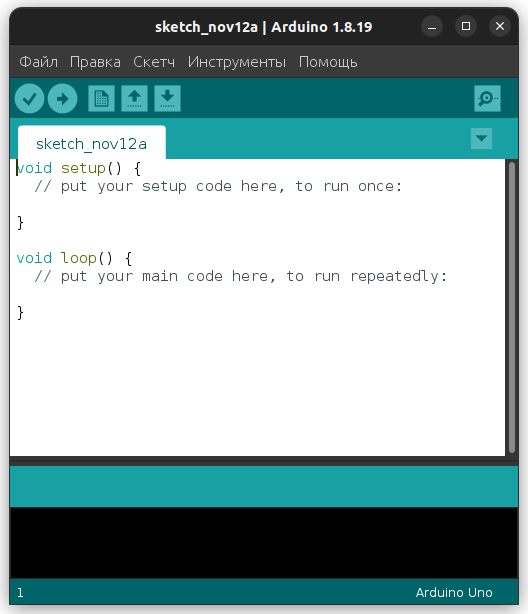
\includegraphics[width=10cm]{arduino-ide-main-window-ru}
  \label{fig:arduino-ide-main-window-ru}
\end{figure}

В англоязычной версии главное окно программы Arduino IDE выглядит, как показано
на рис. \ref{fig:arduino-ide-main-window-en}.

\begin{figure}[ht]
  \centering
  \caption{Главное окно Arduino IDE (английская версия.)}
  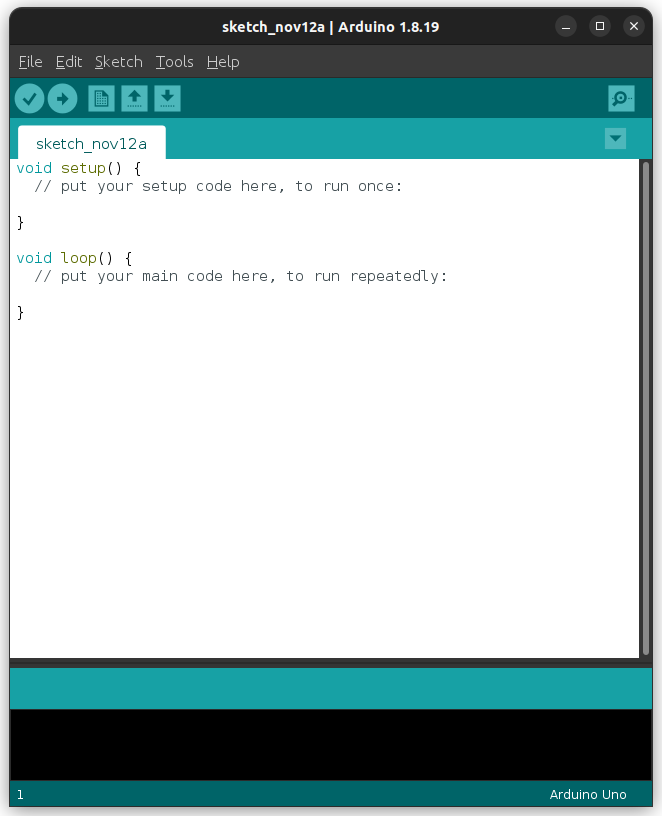
\includegraphics[width=10cm]{arduino-ide-main-window-en}
  \label{fig:arduino-ide-main-window-en}
\end{figure}

Сменить язык интерфейса можно через меню ``Файл'' (``File'') $\rightarrow$
``Настройки'' (``Preferences''), где в открывшемся диалоговом окне необходимо
выбрать из выпадающего списка ``Язык редактора'' (``Editor language'') нужный
вам вариант.

Ниже приведено описание кнопок в интерфейсе Arduino IDE.

%% TODO:

\begin{tabular}{p{4cm}|p{6cm}}
  Название & Описание \\
  \hline \hline
  Verify/Compile (Проверка) & Проверка программного кода. \\
  \hline
  Upload (Загрузка) & Компилирует программный код.\\
  \hline
  New (Создать) & Создание нового скетча.\\
  \hline
  Open (Открыть) & Открыть скетч.\\
  \hline
  Save (Сохранить) & Сохранить скетч.\\
  \hline
  Serial Monitor (Монитор порта) & Открыть монитор порта.\\
\end{tabular}

\section{Основы работы с мультиметром}
Мультиметр -- незаменимый прибор, с его помощью можно узнать сопротивление
резистора, измерить напряжение, произвести проверку на проводимость
(``прозвонка''), узнать цвет и полярность светодиода и многое другое.

На рис. \ref{fig:multimeter-example} показан один из вариантов мультиметра.

\begin{figure}[ht]
  \centering
  \caption{Пример мультиметра.}
  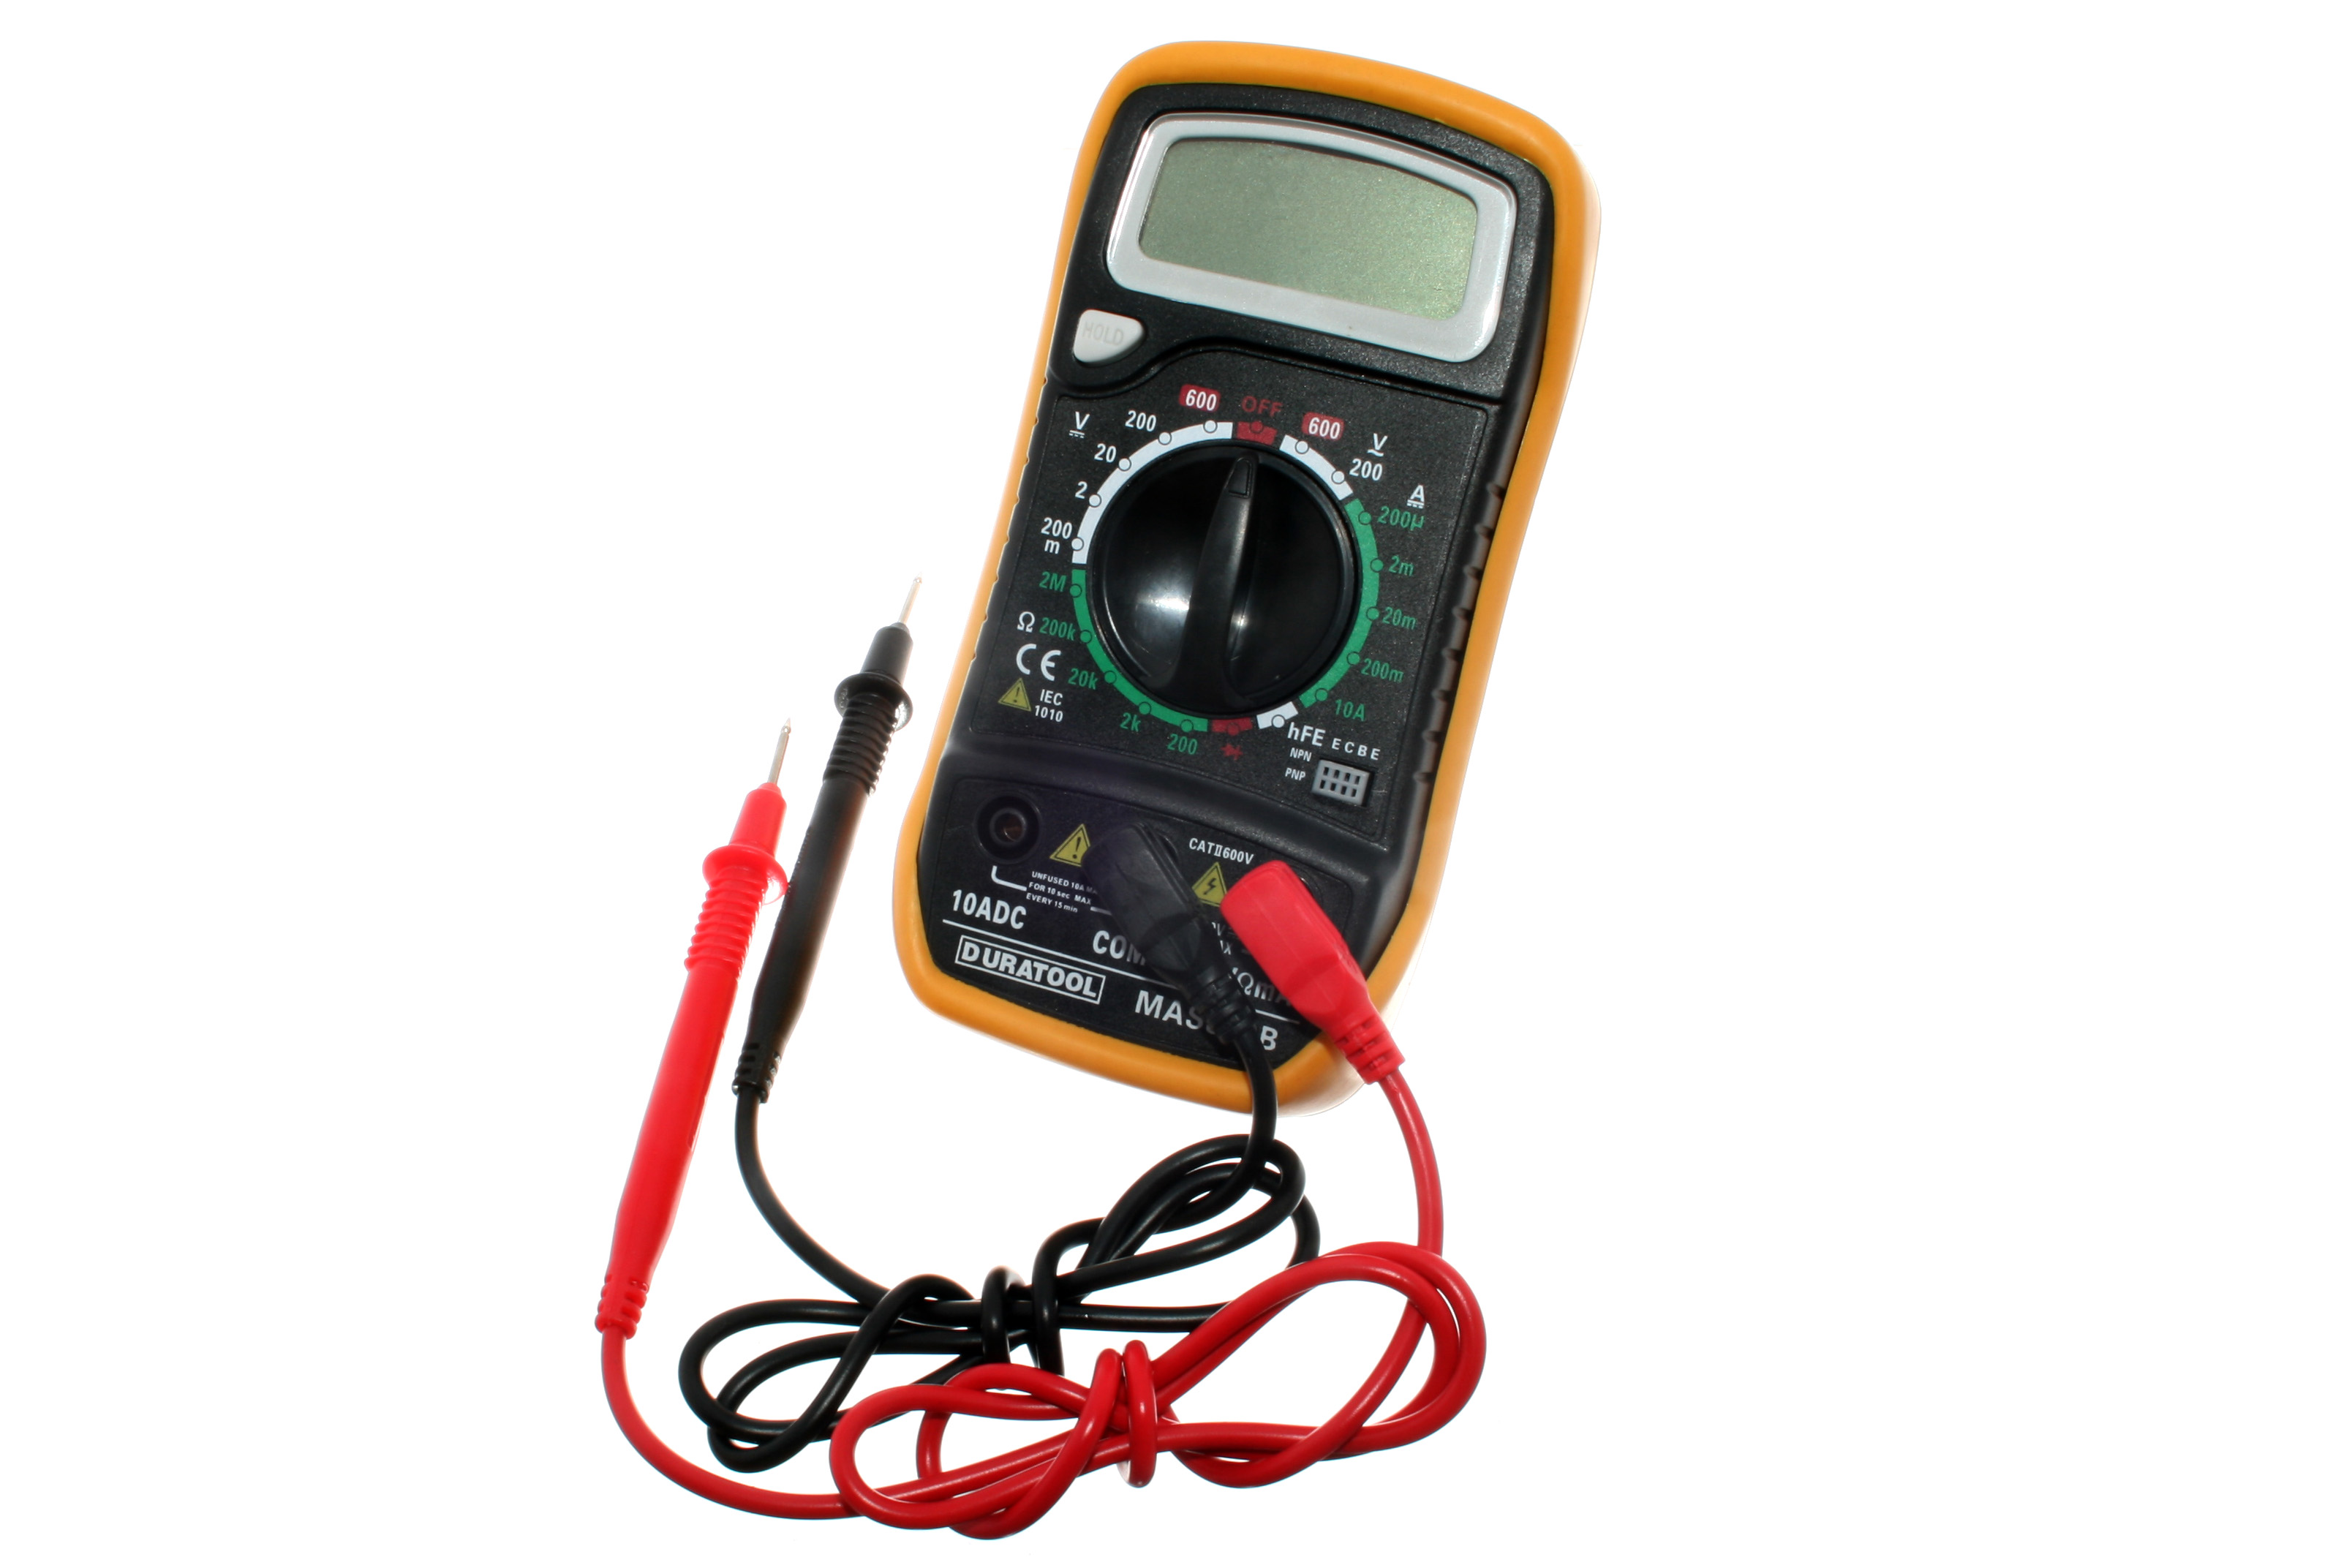
\includegraphics[width=12cm]{Digital_Multimeter}
  \label{fig:multimeter-example}
\end{figure}

Далее приведена таблица на которой отражены основные символы, встречающиеся на
корпусе прибора, необходимые для работы с мультиметром:

\end{document}
